\EXERCISE
شکل زیر را در نظر بگیرید. اگر حرکت تنها در جهت راست و بالا مجاز باشد:
\begin{center}
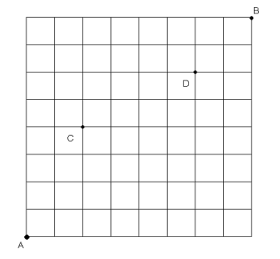
\includegraphics[height=6.5cm]{15.png}
\end{center}
\begin{enumerate}
\item
به چند طریق می‌توان از
$A$
به
$B$
رفت؟
\item
به چند طریق می‌توان با گذشتن از
$C$
و
$D$
از
$A$
به
$B$
رفت؟
\item
به چند طریق می‌توان از
$A$
به
$B$
رفت به‌طوری که نه از
$C$
عبور کنیم و نه از
$D$
؟
\end{enumerate}